
\section{Numerische Integrationsverfahren}
Sei $p$ eine Funktion $p \! : Y \rightarrow p(Y)$, die numerisch über ein
Intervall $[y_1, y_2]$ integriert werden soll.
\begin{equation}
P(y_1, y_2) \; = \; \int\limits_{y_1}^{y_2} \, p(Y) \, \operatorname{d}Y
\end{equation}
Integrieren bedeutet, die Fläche unter der Kurve zu berechnen. Wir approximieren die
Fläche unter der Kurve durch Rechtecke einer festen Breite $\Delta Y$ und einer Höhe
$p(Y_i)$ in der in Abb.~\ref{Trapez} dargestellten Weise.
\begin{figure}
\begin{center}
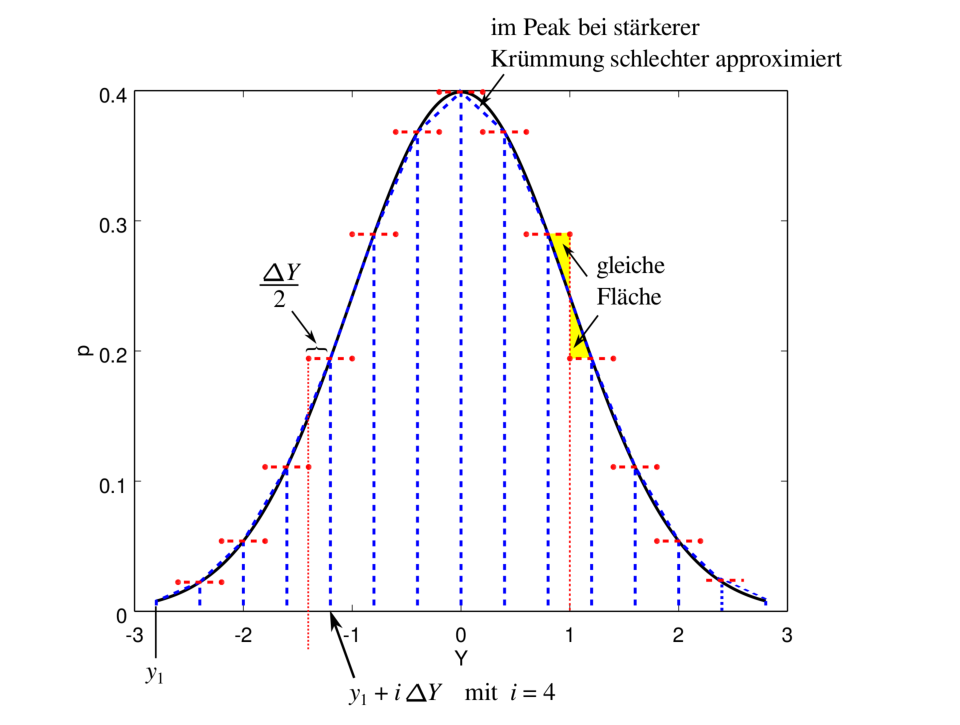
\includegraphics[width=130mm]{07_vorlesung/media/numerischeIntTrapez.pdf}
\caption{\label{Trapez} Trapezapproximation für die Berechnung der Fläche unter einer
Kurve zur numerischen Integration.}
\end{center}
\end{figure}
Die Flächen der mit rot, gestrichpunkteter Linie gekennzeichneten Rechtecke sind genauso
groß wie die mit blau gestrichelter Umrandung markierten Trapezstücke. Diese Flächen
werden summiert, um näherungsweise die Fläche unter der Kurve zu bestimmen.
Das erste und das letzte Flächenstückchen sind nur halb so groß.
Das Integrationsintervall wird in $n$ Flächen unterteilt, so dass für die Breite
der Flächenstücke gelte
\begin{equation}
\Delta Y \; = \; \frac{y_2 - y_1}{n} .
\end{equation}
Es wird nun so aufgeteilt, dass $n-1$ Stücke betrachtet werden gemäß den rot
gestrichpunkteten Rechtecken mit der Breite $\Delta Y$ und zwei weitere Stücken je
der Hälfte dieser Breite und je eines ganz am Anfang und das andere als letztes
Stückchen ganz am Ende.
Das erste Stückchen hat die halbe Breite und die Fläche
$$
\underbrace{\frac{\Delta Y}{2} \, p(y_1)}_{\mathrm{Rechteck}}
 \; + \;
\underbrace{\frac{\Delta Y}{4} \, (p(y_1 + \frac{\Delta Y}{2}) - p(y_1))}_{\mathrm{Dreieck}}
\; = \;
\frac{\Delta Y}{4} \, (p(y_1 + \frac{\Delta Y}{2}) + p(y_1))
$$
das letzte Stückchen analog
$$
\frac{\Delta Y}{4} \, (p(y_2 - \frac{\Delta Y}{2}) + p(y_2))
$$
so dass für die gesamte Fläche gilt
\begin{equation}
P(y_1, y_2) \; = \; \varepsilon \; + \;
\frac{\Delta Y}{4} \, \left(p(y_1 + \frac{\Delta Y}{2}) + p(y_1) +
p(y_2 - \frac{\Delta Y}{2}) + p(y_2)\right) \; + \;
\sum\limits_{i=1}^{n-1} \,
p(y_1 \, + \, i \, \Delta Y) \, \Delta Y
\end{equation}
mit $\varepsilon$ für die Abweichung von der Fläche, die unter der Kurve liegt.
Dabei gilt es eine geeignete Wahl für die Breite $\Delta Y$ der Intervalle
oder andersrum ausgedrückt für die Anzahl $n$ der Intervalle zu treffen.

Eine Möglichkeit ist, sich iterativ zu einer sinnvollen Anzahl von Intervallen
vorzuarbeiten, indem die Intervallbreite $\Delta Y$ mit jedem Iterationsschritt halbiert wird.
Dabei arbeitet man sich solange vor bis sich die approximierte Fläche
durch weiteres Halbieren der Intervallbreiten nicht mehr
signifikant ändert. Diese Methode wird \textsl{Romberg}-Verfahren genannt.
Werner Romberg war ein in Berlin geborener Mathematiker, der in Heidelberg und München
studierte und promovierte. Kurz nach dem Rigorosum im Jahr 1933 musste er als Kritiker
des Nazionalsozialismus Deutschland verlassen. 1949 wurde Werner Romberg Dozent für Physik
am Norwegian Institute of Technology (NTH) in Trondheim und richtete dort den Studiengang
für Mathematische Physik ein. 1955 publizierte er dieses numerische Integrationsverfahren.

Ein Quellcode-Beispiel in C ist auf der Wikipediaseite zum Romberg-Verfahren zu finden:
\begin{verbatim}
https://en.wikipedia.org/wiki/Romberg%27s_method
\end{verbatim}
Bei jedem Iterationsschritt wird $\Delta Y$ halbiert.
Der Iterationsschritt $n = 1$ bedeutet $\Delta Y_1 = y_2 - y_1$, Schritt $n = 2$
bedeutet $\Delta Y_2 = (y_2 - y_1)/2 = \Delta Y_1/2$ etc.
\begin{equation}
P_n (y_1, y_2) \; = \;
\frac{\Delta Y_n}{4} \, (p(y_1 + \frac{\Delta Y_n}{2}) + p(y_1) +
p(y_2 - \frac{\Delta Y_n}{2}) + p(y_2)) \; + \;
\sum\limits_{i=1}^{n-1} \,
p(y_1 \, + \, i \, \Delta Y_n) \, \Delta Y_n
\end{equation}
mit
$$
 \Delta Y_n \, = \, \frac{1}{2} \Delta Y_{n-1} .
$$
Die Iteration endet, sobald der Betrag der Differenz der approximierten Flächen
\begin{equation}
\mid P_n (y_1, y_2) \, - \, P_{n-1} (y_1, y_2) \mid \, < \, \varepsilon_P
\end{equation}
einen Wert annimmt, der kleiner als ein zuvor definierter sehr kleiner Wert $\varepsilon_P$ ist.

Dabei werden die Flächenstücke durch Halbierung der Intervallbreite gleichförmig schmaler gemacht.
Die einzelnen Abweichungen zu jedem der Intervalle können für unterschiedlich stark gekrümmte
Segmente der unterschiedlichen Stückchen verschieden groß sein, so dass für manche
Anwendungen dadurch Rechenzeit gesparen werden, dass nur ausgewählte Bereiche
verfeinert werden. Hier ist mehr Aufwand bei der Implementierung der Verästelung des Baumes,
der für unterschiedlichen Integrationsbereiche unterschiedliche Iterationstiefen verwaltet,
erforderlich. Wir nennen die Grenzen der Flächenstückchen, die bei Romberg gleichförmig die Positionen
$$
Y_i \, = \, y_1 \, + \, (i-1) \Delta Y
$$
annehmen, \textsl{Samples}, für die im allgemeinen gelten kann
\begin{equation}
Y_{i+1} - Y_i \, \neq \, Y_{k+1} - Y_k \quad \mathrm{f{"u}r} \quad i \neq k .
\end{equation}

%Ein Maß dafür, um wieviel die trapezförmigen Flächenstücke zu
%groß oder zu klein sind, ist beispielsweise der Abstand $\delta_i$
%zwischen der jeweiligen Sekante und dem Wert
%der Funktion $p$ in der Mitte der Sekante (blau gestrichelte Linien)
%\begin{equation}
%\delta_i \; = \; p(y_1 \, + \, i \Delta Y \, - \, \frac{\Delta Y}{2}) \; -
%\; \frac{1}{2} \left( p(y_1 \, + \, i \Delta Y) +  p(y_1 \, + \, (i-1) \Delta Y ) \right) .
%\end{equation}
%Bei Funktionsverläufen mit relativ gleichförigem Krümmungsverhalten wird
%ein integrales Maß aus den $\delta_i$ verwendet, um zu bewerten ob sich bei feinerer

Insbesondere bei der Integration mehrdimensionaler Funktionen, wie wir sie
in unseren Bespielen hatten, bevor wir die Marginalverteilung erworben hatten,
also soetwas wie bei folgender Integration
$$
\int\limits_{-\infty}^\infty \cdots \int\limits_{-\infty}^\infty
p(Y, X_1, \dots, X_N | \{X_{i,1}, \dots, X_{i,J_i}\}, \bar x_k, s_k, \dots)
\operatorname{d}X_1 \dots \operatorname{d}X_N
$$
gilt es die \textsl{Samples} für die Hypervolumenstückchengrenzen optimal zu wählen.
Die Berechnungen sollen in minimaler Zeit fertig werden und dennoch soll das
gesamte Hypervolumen möglichst genau approximiert werden.

Betrachten wir konkret die Aufgabe, Wahrscheinlichkeitsdichteverteilungen $p$
integrieren zu wollen, welche dadurch gekennzeichnet sind, dass ihre Funktionswerte
positiv sind und dass sie aus einem
oder vielleicht auch ganz wenig mehr als einem breiteren \textsl{Peak} (Glocke) bestehen.
Diese Glocke muss dabei nicht unbedingt so schön symmetrisch sein wie bei der
Normalverteilung oder bei der Student-t-Verteilung, sondern kann eine gewisse Schiefe haben
wie beispielsweise bei der $\chi^2$-Verteilung für wenige Freiheitsgrade.
Wenn wir Abb.~\ref{Trapez} genauer anschauen, sehen wir, dass die Sekanten im Zentrum
des \textsl{Peaks}, der Glocke, stärker von der Kurve der Glocke abweichen als in den
\textsl{Tails}. Die Sample-Stützstellen wollen wir also im Bereich des Glockenmaximums, bzw.\
in den Bereichen der Glockenmaxima, enger legen als in den \textsl{Tails}. Dies ist äquivalent
zu dem, die Dichte der Stützstellen gemäß der Verteilung $p$ selbst zu samplen.
Mit anderen Worten, es wird eine nach $p$ verteilte Stichprobe der Größen $X_i$
entnommen. Die Verteilung $p$ wird verwendet, um gleichverteilte Pseudozufallszahlen auf nach $p$
verteilte Zahlen abzubilden.
Dieser Ansatz liegt den sogenannten \textsl{Importance Sampling}-Algorithmen zugrunde.

Wenn eine Verteilung $p$ stark fluktuiert, also innerhalb eines
Intervalls (des $i$-ten Intervalls) auf der $X$-Achse sehr unterschiedliche Funktionswerte $p(X_i)$ annimmt,
so bedeutet das, dass $p(X_i)$ eine große Varianz hat.
\begin{equation}
\operatorname{Var}(p(X_i)) \; = \; \frac{1}{J-1} \sum_{j=1}^J \, \left(p(X_{i,j})- \bar p(X_i)\right)^2 .
\end{equation}
Die Varianz bezüglich unterschiedlicher Intervalle, bzw.\ Regionen, wird als Maß verwendet,
das der Entscheidung zugrunde gelegt wird, ob weitere Stützstellen in dieser Region
gesampelt werden, die Region in kleinere Regionen zu unterteilen, um je Region kleinere Varianzen
zu erhalten.
Das Sampeln innerhalb der verschiedenen Regionen geschieht dabei
voneinander unabhängig. Die Regionen werden auch Gruppen oder Schichten genannt.
Ein nach diesem Verfahren gebildetes Sample heißt \textsl{geschichtete Zufallsstichprobe}
oder \textsl{stratifizierte Zufallsstichprobe} (engl.\ \textsl{stratified Sample}).

\section{Zufallszahlen und Wahrscheinlichkeitsverteilungen}
Die Thematik des Samplings nach Methoden, bei denen Zufallszahlen verwendet werden, ist ein
weites Feld in der Statistik. Große Bedeutung haben zufallszahlenbasierte Integrationsmethoden,
die auf Erkenntnissen aus der Thermodynamik, d.h.\ der statistischen Physik beruhen.
Sie wurden aus Beobachtung der brown'schen Molekularbewegung abgeleitet, also aus der
Zufälligkeit und Art und Weise der Bewegung von Molekülen eines Fluids.
Der zurückgelegte Pfad eines Moleküls, \textsl{Random Walk},
ändert zufällig die Richtung.
%, aber die Einzelpositionen haben eine gewisse Autokorrelation.

Die Abfolge der Transformationen, die eine aktuelle Position eines Gegenstands oder den
aktuellen Zustand eines Prozesses in die nachfolgende Position bzw.\ den nachfolgenden
Zustand überführt, und daraus die danach nachfolgende Position (den daraus folgenden Zustand)
und so weiter, heißt \textsl{Markow-Kette}. Kennzeichen einer Markow-Kette ist, dass die
Positions\-änder\-ung des Moleküls nur von der aktuellen Position,
nicht aber von den Positionen davor, abhängt. Allgemein lassen sich viele statistische Prozesse,
nicht nur Pfade von Fluidpartikeln oder Abfolgen der Werte von Zufallssampeln, mit Hilfe von
Markow-Ketten beschreiben und es gilt:
\begin{quote}
Der zukünftige Zustand des Prozesses ist nur durch den
aktuellen Zustand bedingt und wird nicht durch vergangene Zustände beeinflusst.
\end{quote}

Um rechentechnisch mit Zufallszahlen zu arbeiten, müssen diese synthetisch generiert werden.
Synthetisch gerechnete Zufallszahlen beruhen auf definierten Algorithmen und
sind deshalb nicht wirklich zufällig, sondern deterministisch. Sie werden deshalb
\textsl{Pseudozufallszahlen} genannt.
Ein deterministischer Algorithmus berechnet eine Zahlenfolge, die nur den
Anschein hat, dass die Zahlenwerte zufällig verteilt sind und nicht deterministisch.

Prinzipiell ist ein solcher Algorithmus, oftmals Zufallszahlengenerator genannt, wie
folgt aufgebaut.
\begin{enumerate}
\item Setzen eines Startwertes, der \textsl{Seed} genannt wird, was ein englischsprachiger
  Begriff ist und Saat, Samenkorn heißt.
\item Wechselweise Multiplikationen und Restklassenoperationen mit sehr großen natürlichen Zahlen, wobei
  bei der Restklassenoperation als Teiler eine möglichst große Primzahl, beispielsweise
  16807, zum Einsatz kommt.
\end{enumerate}
Mit Restklassenoperation ist hier gemeint, dass eine Division mit natürlichen Zahlen
durchgeführt wird, deren Rest als Ergebnis in die weiteren Berechnungsschritte eingeht.


\begin{figure}
\begin{center}
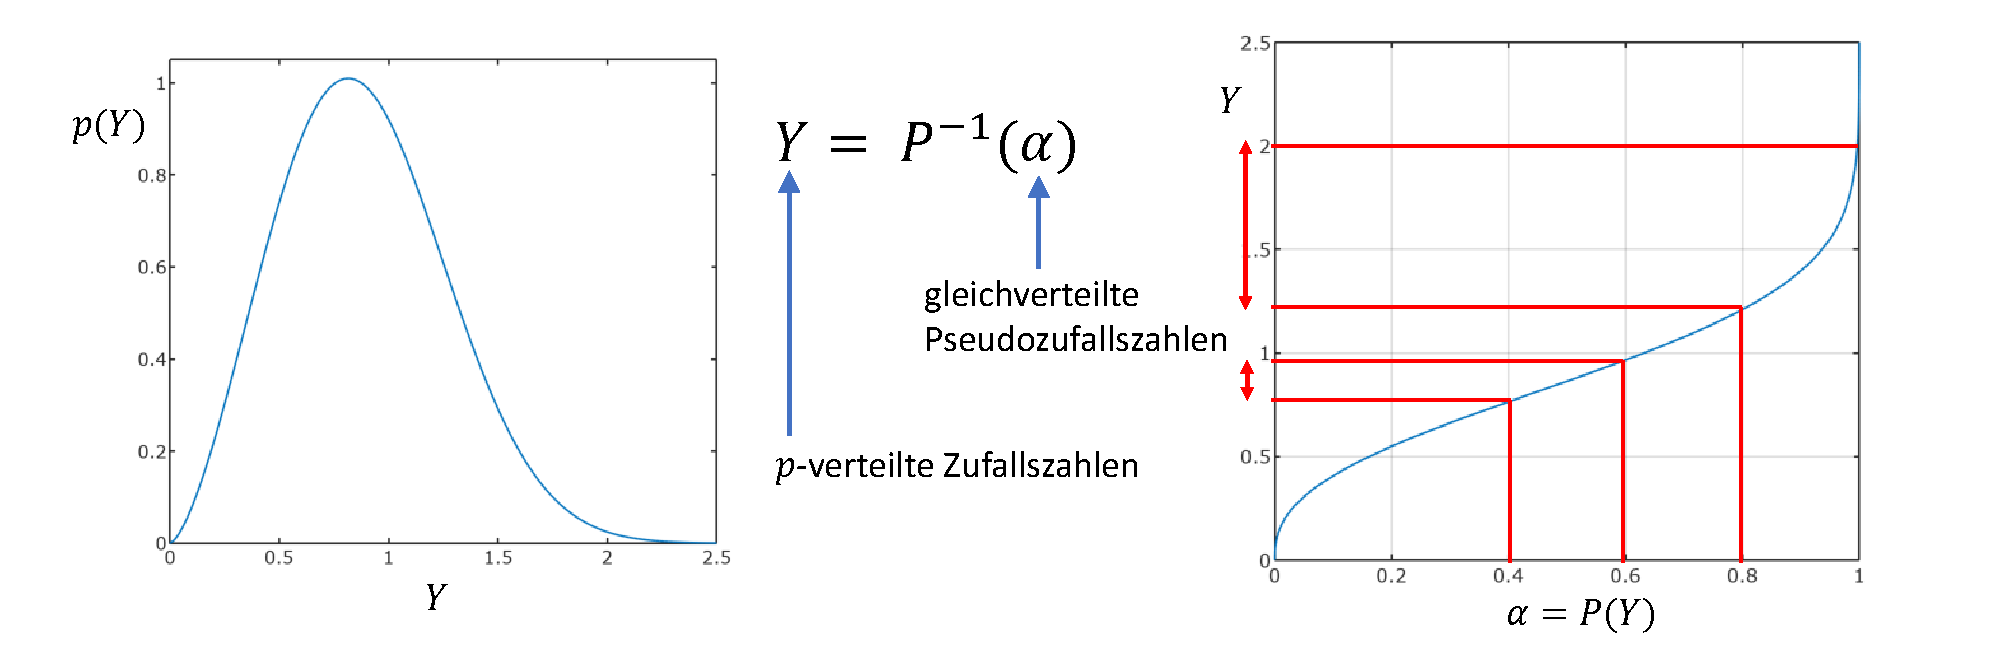
\includegraphics[width=160mm]{07_vorlesung/media/TransformRandomDistri.pdf}
\caption{\label{pverteilteZufallszahlen} Eine gleichverteilte Größe wie beispielsweise
eine Wahrscheinlichkeit $\alpha$ wird über die inverse Funktion $P^{-1}$ der
kummulierten Wahrscheinlichkeitsverteilung $P$, also der aufintegrierten Verteilung
der Wahrscheinlichkeitsdichte $p$, abgebildet auf die Größe $Y$, die dann $p$-verteilt ist.}
\end{center}
\end{figure}
Die heutigen Bibliotheken für Compiler und Programmiertools wie Matlab bieten nicht nur
Zufallszahlengeneratoren, die gleichverteilte Zahlenfolgen liefern. Sie stellen schon
fertige, schnelle, effektive Algorithmen zur Verfügung, die die Transformation auf die üblichen
Verteilungsdichtefunktionen $p$ zur Verfügung stellen. So ist \texttt{randn} der Name der Funktion
in Matlab und Gnu-Octave zur Erzeugung von normalverteilten Zufallszahlen. \texttt{rande}
liefert exponentiell verteilte Zufallszahlen, \texttt{randg} Zufallszahlen, die nach
der Gammafunktion verteilt sind und \texttt{randp} poissonverteilte Zufallszahlen. In Python sind
diese in der zu \texttt{numpy} gehörenden Biblothek \texttt{random} zu finden. Mit
\texttt{randn} werden standardnormalverteilte Zufallszahlen erzeugt:
%\lstset{language=Python}
\begin{lstlisting}[style=Python]
import numpy as np
nrow = 5
ncol = 20
a = np.random.randn(nrow, ncol)
\end{lstlisting}
Mit \texttt{rand} werden gleichverteilte Zufallszahlen $R \in [0, 1)$ erzeugt.

Wir können aber auch selber gleichverteilte Zufallszahlen abbilden auf eine andere Verteilung $p$,
wenn wir die Umkehrfunktion der kumulierten Verteilung $P^{-1}$ dazu zur Verfügung haben.
Sei $R = \{R_1, \dots, R_J\}$ ein Sample, eine Stichprobe, gleichverteilter Zufallszahlen mit
$R \in [0,1)$, so ist die Menge der mit $P^{-1}$ transformierten Zufallszahlen
$$
Z \; = \; P^{-1}(R)
$$
gemäß $p$ verteilt, siehe Abb.~\ref{ZufallszahlenAbbilden}.

Als Beispiel wollen wir in Python 1000 Zufalls\-zahlen generieren,
die verteilt sind gemäß einer $t$-Verteilung für 45 Freiheitsgrade:
%\lstset{language=Python}
\begin{lstlisting}[style=Python]
import numpy as np
import scipy
from scipy import stats
Jz = 1000
nu = 45
R = np.random.rand(1, Jz)
Z = scipy.stats.t.ppf(R[0], nu)
\end{lstlisting}

\section{Monte-Carlo-Verfahren gemäß GUM-supplement~1 JCGM 101}

In Kapitel~\ref{montecarloMU} werden wir das Monte-Carlo-Verfahren gemäß GUM-supplement~1 JCGM 101
erläutern, bei dem wie oben bereits erwähnt,
gemäß den jeweiligen Ver\-teil\-ungen der unterschiedlichen direkten Messgrößen
eine große Stichprobe (ein großes \textsl{Sample})
$\mathbf{x}_1 = (x_{1,1},\dots,x_{N,1})^\mathsf{T}$, $\dots$, $\mathbf{x}_J = (x_{1,J},\dots,x_{N,J})^\mathsf{T}$
für die direkten Größen $\mathbf{X}$ per Zufallszahlengenerator erzeugt
wird. Diese wird in das Modell $f$ gesteckt,
um eine Stichprobe
\begin{equation}
y_1 = f(x_{1,1},\dots,x_{N,1}), \dots, y_J = f(x_{1,J},\dots,x_{N,J})
\end{equation}
der indirekten Größe $Y$ zu gewinnen. Entweder wird aus der inversen Funktion der kumulierten
Wahrscheinlichkeitsverteilung das Überdeckungsintervall gewonnen oder es werden aus dem Sample $y_1,\dots, y_J$
der Erwartungswert $\bar y$ und die Standardabweichung $\sigma_Y$ gemäß
$$
\bar y = \frac{1}{J} \sum_{j=1}^{J} y_j \qquad
\sigma_Y = \sqrt{\frac{1}{J-1} \sum_{j=1}^{J} (y_j - \bar y)^2}
$$
berechnet.

Dieses Verfahren entspricht gemäß \cite{Wue08} in etwa den Berechnungen wie
in Gl.~(\ref{PosteriorSensor}), nämlich wenn wir für die Standardabweichung $\sigma_\mathrm{winzig}$
den Grenzübergang $\sigma_\mathrm{winzig} \rightarrow 0$ machen, sodass die zu integrierende
Verteilung in die folgende übergeht:
\begin{equation}
\arraycolsep=2.0pt\def\arraystretch{2.0}
\begin{array}{l}
p(Y, X_\mathrm{K}, X_\mathrm{M} | (X_{\mathrm{M},1}, \dots, X_{\mathrm{M},J}), K_0, s_\mathrm{K}) \propto \\
\delta\left(Y \; - \; X_\mathrm{K} \, X_\mathrm{M}\right)
\;  e^{-\frac{1}{2} \left(\frac{X_\mathrm{K} - K_0}{s_\mathrm{K}} \right)^2} \; \prod\limits_{j=1}^J  \,
e^{-\frac{1}{2} \left(\frac{ X_\mathrm{M} - X_{\mathrm{M},j} }{s_\mathrm{M}} \right)^2}
\end{array}
\label{PosteriorFall4}
\end{equation}
Zu den Größen $X_\mathrm{K}$ und $X_\mathrm{M}$ werden dann zufällige
Samples gewählt.

Im folgenden werden wir den Grenzübergang der Wahrscheinlichkeitsdichte für das Modell
\begin{equation}
\lim_{\sigma \rightarrow 0} \left\{ e^{-\frac{1}{2} \left(\frac{Y-f(\mathbf{X})}{\sigma}\right)^2} \right\}
= \delta\left(Y \; - \;f(\mathbf{X})\right)
\end{equation}
in eine dirac'sche Distribution als \textsl{scharfen Modellprior} bezeichnen.

Für univariate, explizite Modellfunktionen und für normalverteilte Größen $X_i$ sieht die
Posterior mit \textsl{scharfem Modellprior} dann wie folgt aus
\begin{equation}
\arraycolsep=2.0pt\def\arraystretch{2.0}
\begin{array}{l}
p(Y, X_\mathrm{1}, \dots, X_\mathrm{N} | (X_{1,1}, \dots, X_{1,J_1}), ..., (X_{K,1}, \dots, X_{K,J_1}),
 \bar x_{K+1}, s_\mathrm{K+1}, \dots, \bar x_{N}, s_\mathrm{N}) \propto \\
\delta\left(Y \; - \; f(X_1, \dots \, X_N)\right)
\; \left( \prod\limits_{i=1}^K \, \prod\limits_{j=1}^{J_i}  \,
e^{-\frac{1}{2} \left(\frac{ X_i - X_{i,j} }{s_i} \right)^2} \right)
\;  \left( \prod\limits_{i=K+1}^N \,  e^{-\frac{1}{2} \left(\frac{X_i - \bar x_i}{s_i} \right)^2} \right) .
\end{array}
\label{PosteriorFall4allgemeiner}
\end{equation}


Wir hatten bereits angesprochen, dass die Monte-Carlo-Verfahren auch insbesondere
für Messaufgaben eingesetzt werden, bei denen mindestens ein Teil der direkten Messgrößen nicht normalverteilt ist.
Dies kann vielfach sein, dass $t$-Verteilungen zu betrachten sind. Es kommen auch immer wieder Messaufbauten
vor, bei denen die U-Verteilung eine Rolle spielt, also keine Glocke, sondern
eine Verteilung, die ihre starken \textsl{Peaks} an den Rändern des Bereichs hat. Dies ist beispielsweise der
Fall für Größen, deren Streuung durch Vibrationen verursacht wird. Die U-förmige Gestalt der Verteilung entspricht dann
dem Quadrat eines Arkussinus.

Anstelle der Gaußfunktionen in Gl.~(\ref{PosteriorFall4allgemeiner}) schreiben wir jetzt
ganz allgemein $p_i$
\begin{equation}
\arraycolsep=2.0pt\def\arraystretch{2.0}
\begin{array}{l}
p(Y, X_\mathrm{1}, \dots, X_\mathrm{N} | (X_{1,1}, \dots, X_{1,J_1}), ..., (X_{K,1}, \dots, X_{K,J_1}), \,
 \theta_{K+1,1}, \dots, \theta_{N,M_K}) \propto \\
\underbrace{\delta\left(Y \; - \; f(X_1, \dots \, X_N)\right)}_{\mathrm{scharfer~Modellprior}}
\; \underbrace{ \left( \prod\limits_{i=1}^K \, \prod\limits_{j=1}^{J_i}  \, p_i (X_{i,j} | X_i) \right) }_{\mathrm{Likelihood}}
\; \underbrace{ \left( \prod\limits_{i=K+1}^N \,  p_i (X_i | \theta_{i,1}, \dots, \theta_{i,M_i}) \right) }_{\mathrm{Prior}} .
\end{array}
\label{PosteriorFall4p}
\end{equation}
mit der Symmetrieeigenschaft $p(X_{i,j} | X_i) = p(X_i | X_{i,j}) \equiv l(X_i | X_{i,j})$.
Dabei stellen $\theta_{K+1,1},$ $\dots,$ $\theta_{N,M_K}$ Parameter aus {\`a} priori Informationen dar,
wie beipielsweise $\theta_{i,1} = \bar x_i$ und $\theta_{i,2} = s_i$.

\begin{figure}
\begin{center}
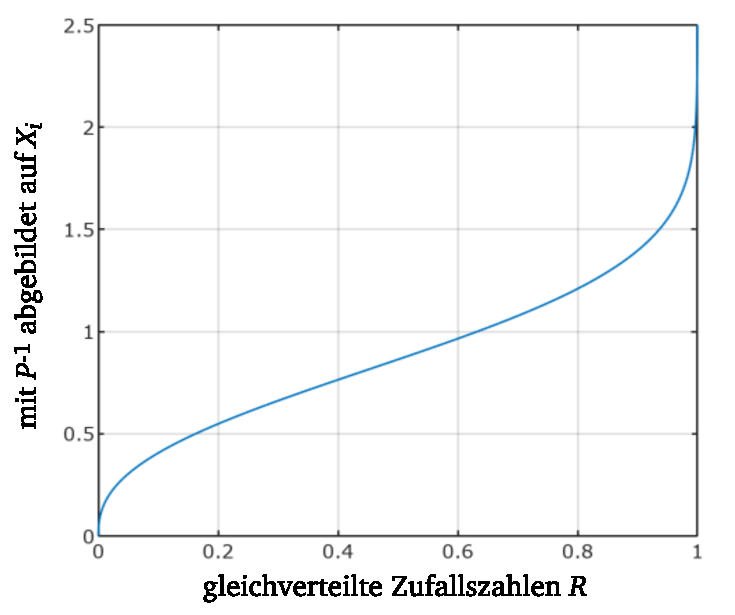
\includegraphics[width=90mm]{07_vorlesung/media/Zufallszahlen_abbilden_Verteilung.pdf}
\caption{\label{ZufallszahlenAbbilden} Ein Sample gleichverteilter Zufallszahlen
$\boldsymbol R = \{R_1, \dots, R_L\}$ wird über die inverse Funktion $P^{-1}$ der
kumulierten Wahrscheinlichkeitsverteilung $P$ abgebildet auf ein
Sample $\boldsymbol X = \{X_1, \dots, X_L\}$, deren Werte dann $p$-verteilt sind.}
\end{center}
\end{figure}
Wie in Abb.~\ref{ZufallszahlenAbbilden} dargestellt wird zur Erzeugung jeder der Verteilungen
$p_i (X_{i,j} | X_i)$ bzw.\ $p_i (X_i | \theta_{i,1},$ $\dots,$ $\theta_{i,M_i})$ der jeweiligen Größe
$X_i$ je ein Sample gleichverteilter Zufallszahlen $\boldsymbol R_i =$ $\{R_{i,1},$ $\dots,$ $R_{i,L}\}$ generiert, das
dann mit $P_i^{-1}$ abgebildet wird auf $\boldsymbol X_i = \{X_{i,1}, \dots, X_{i,L}\}$.
Wir wissen, dass die $X_{i,j}$ beobachtete Werte der Größe sind, also Konstanten, die die Funktion
$P_i^{-1}$ parametrisieren. Entsprechend sind auch die $\theta_{i,1}, \dots, \theta_{i,M_i}$ Konstanten, die
die dazugehörige Funktion $P_i^{-1}$ parametrisieren. $\theta_{i,m}$ sind beispielsweise Mittelwert und
Standardabweichung, oder andere Modellparameter, die aus Beobachtungen (Messdaten) gewonnen wurden.
Zu jeder der Funktionsvariablen $X_i$ wird also wie soeben beschrieben jeweils ein Sample $p_i$-verteilter
Zufallsgrößen generiert. Für die Samples wird jeweils derselbe Stichprobenumfang $L$ gebraucht, damit
sich Tupel $(X_{1,l}, \dots, X_{N,l})$ mit $l = 1,\dots, L$ zusammenstellen lassen, aus denen über die
Modellfunktion $f$ jeweils der Wert $Y_l$ für die indirekte Messgröße $Y$ berechnet wird
\begin{equation}
Y_l \; = \; f(X_{1,l}, \dots, X_{N,l})
\end{equation}
mit $L$ eine sehr große natürliche Zahl.

Aus der Verteilung der Werte $Y_l$ lässt sich dann die Messunsicherheit bestimmen.
Dieses Verfahren wird angewendet, wenn sich keine Sensitivitätskoeffizienten zu $f$
berechnen lassen oder wenn die Sensitivitätskoeffizienten in der Nähe von Null liegen, weil
$f$ in der Umgebung der Schätzwerte ganz flach ist, also ein Extremum oder Sattelpunkt hat.
Das bedeutet, dass $f$ nicht linearisierbar ist.

Insbesondere wird das Verfahren mit den großen Zufallszahlensamples dann angewendet, wenn es
keine analytisch geschlossene Darstellung zu dem Modell $f$ gibt.
Numerische Verfahren unter Anwendung von Zufallszahlen werden häufig in Anlehnung an den Zufall
des Würfel- oder Roulettespiels Monte-Carlo-Verfahren genannt, so auch hier bei der Ermittlung
von Messunsicherheiten.
